% !TEX root = ../ITGO.tex

\subsection*{Gear train design problem}

In this problem, the objective is to minimize the cost of the gear ratio of the gear train \citep{PV}. An example is shown in Figure \ref{fig:GT}. The problem has four variables, representing the number of teeth for the four gears ($x_1 = A$, $x_2 = B$, $x_3 = D$, and $x_4 = F$), with $f(\bm{x}^*) = 2.700857E \! - \! 12$. The only constraint of the problem is that all variables must be integers.


\begin{figure}[h]
    \begin{center}
    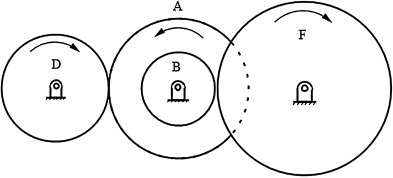
\includegraphics[scale=0.6]{Imgs/GT.jpg}
    \end{center}
    \captionsetup{justification=centering}
    \caption{Gear train design problem structure.}\label{fig:GT}
\end{figure}

\prob{Appendix/Problems/GT}